\documentclass[tikz,border=10pt]{standalone}
\usepackage{amsmath}

% 使用 tikz 宏包
\usetikzlibrary{arrows.meta, calc}

\begin{document}

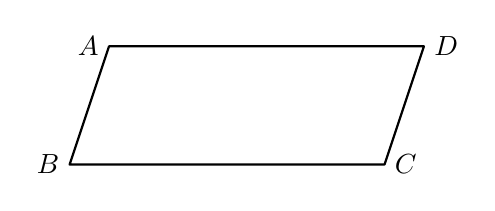
\begin{tikzpicture}[thick, line join=round, line cap=round]
    % --- 1. 参数定义 ---
    \def\w{4}     % 平行四边形的宽度 (BC 长度)
    \def\h{1.5}   % 平行四边形的高度
    \def\off{0.5} % A点相对于B点的水平偏移量 (控制倾斜度)

    % --- 2. 坐标设定 ---
    \coordinate (B) at (0, 0);
    \coordinate (C) at (\w, 0);
    \coordinate (A) at (\off, \h);
    \coordinate (D) at ({\w+\off}, \h);

    % --- 3. 绘制平行四边形边界 ---
    \draw (A) -- (B) -- (C) -- (D) -- cycle;

    % --- 4. 顶点标注 ---
    % anchor 用于微调文字相对于坐标点的方向
    \node[left]  at (A) {$A$};
    \node[left]  at (B) {$B$};
    \node[right] at (C) {$C$};
    \node[right] at (D) {$D$};

\end{tikzpicture}

\end{document}